\documentclass[12pt, openany]{report}
%\usepackage[latin1]{inputenc}
\usepackage[utf8]{inputenc}
\usepackage[T1]{fontenc}
\usepackage[a4paper,left=2cm,right=2cm,top=2cm,bottom=2cm]{geometry}
\usepackage[frenchb]{babel}
\usepackage{libertine}
\usepackage{titlesec}
\usepackage{lipsum}
\usepackage{scrextend}
\usepackage[pdftex]{graphicx}
\usepackage{tabularx}
\usepackage{float, caption}
\usepackage{colortbl}
\usepackage{array}
\usepackage{verbatim}
\usepackage{fancyvrb}


%Réglage de l'espacement pour les chapitres
\titleformat{\chapter}[display]   
	{\normalfont\huge\bfseries}{\chaptertitlename\ \thechapter}{5pt}{\Huge}  
\titlespacing*{\chapter}{0pt}{-30pt}{5pt}


\setlength{\parindent}{0cm}
\setlength{\parskip}{1ex plus 0.5ex minus 0.2ex}
\newcommand{\hsp}{\hspace{20pt}}
\newcommand{\HRule}{\rule{\linewidth}{0.5mm}}

\newenvironment{indentpar}[1]%
  {\begin{list}{}%
          {\setlength{\leftmargin}{#1}}%
          \item[]%
  }
  {\end{list}}

\begin{document}


\begin{titlepage}

\includegraphics[width=5cm]{upmc.png}
\begin{sffamily}
\begin{center}
% Mise en place de l'image
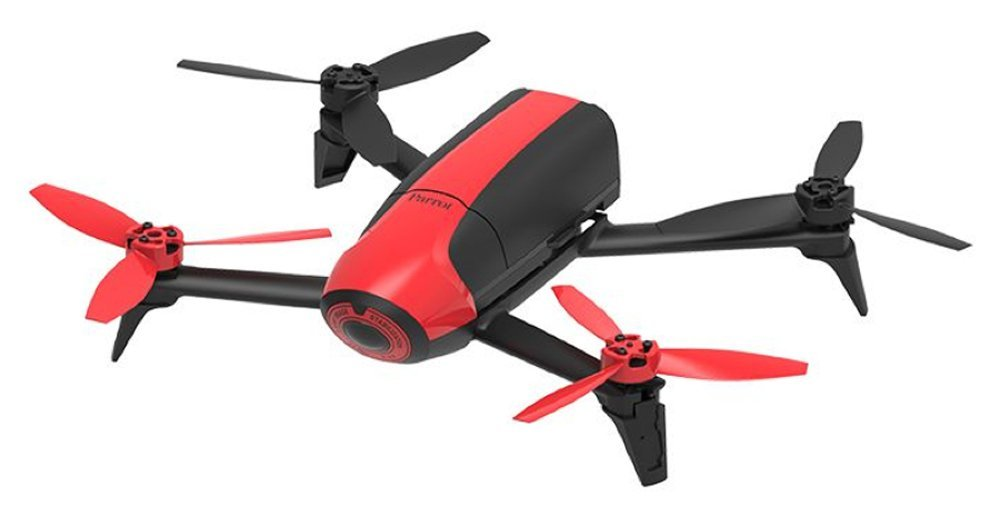
\includegraphics[scale=0.4]{img1.jpg}~\\[1cm]
\textsc{\Large Projet : DRONE AUTOPILOT}\\[1cm]

% Titre
\HRule \\[0.4cm]
	 { \huge \bfseries Cahier des charges\\[0.4cm] }
 \HRule \\[2cm]
 
 \textsc{\LARGE Université Pierre et Marie Curie}\\[3cm]

 % Auteurs et tuteur
\begin{minipage}{0.4\textwidth}
\begin{flushleft} \large
Axel \textsc{Archambault}\\
Yoann \textsc{Ghigoff}\\
Nicolas \textsc{Salleron}\\	%Sens Alphabétique
Kévin \textsc{Vu-Saintonge}\\
\end{flushleft}
\end{minipage}
\begin{minipage}{0.4\textwidth}
\begin{flushright} \large
\emph{Tuteur :} M. Fabrice \textsc{Kordon}\\
-\today
\end{flushright}
\end{minipage}

\vfill

\end{center}
\end{sffamily}
\end{titlepage}


%Mise en place du sommaire
\tableofcontents


%%%%%% INTRODUCTION %%%%%%
%Précise l'objectif du document et en résume le contenu

\chapter{Introduction}
\paragraph{}
Utilisés depuis les années 1990 dans le cadre militaire, les drones font aujourd'hui partie de notre vie de tous les jours. Des sociétés comme Parrot les ont popularisé au sein du grand public. Les smartphones étant de plus en plus répandus et performants, les applications peuvent exploiter les multiples capacités de leurs capteurs embarqués. Les progrès de la miniaturisation permettent même l'utilisation de ces technologies dans de plus petits objets connectés tels les montres.\\
Les drones sont très souvent utilisés, notamment dans les domaines artistiques comme la danse. Des émissions en témoignent : "La France a un incroyable talent" (25/10/2016) et "Britain's got talent", outre-Manche.\\À Las Vegas, durant le CES 2016, la société Parrot a réalisé le "Drone dance" dans lequel les drones Parrot "dansent" de manière autonome sur une chorégraphie pré-enregistrée. A Londres la même année, la société BeTomorrow a présenté le "Flying Oreo show". 
Nous observons un réel intérêt du grand public pour les drones et la démonstration de leurs capacités à travers le spectacle et la danse.

\section{Contexte}
\paragraph{}
Notre projet d'"\textit{Ingénierie Dirigée par les modèles}" est inscrit dans le domaine de la danse. Un danseur doit être capable de préparer la chorégraphie puis de l'exécuter sur le terrain de son choix. L'utilisateur utilisera pour ce faire un langage de programmation spécifique que nous allons réaliser afin de préparer ses danses simplement. 

\section{Objectifs}
\paragraph{} L'objectif est de permettre à un danseur de réaliser une chorégraphie. Pour ce faire notre équipe produira un langage de programmation simple et compréhensible pour l'utilisateur. \\Ce dernier devra par la suite l'utiliser de manière autonome afin de préparer en amont la chorégraphie de son drone. Une fois la chorégraphie validée et compilée par notre logiciel frontal, l'utilisateur doit pouvoir lancer l'application générée par notre frontal. Cette application enverra différents ordres au drone et réalisera la chorégraphie.

\chapter{Le langage de pilotage du drone}

Notre solution sera un langage avec une syntaxe textuelle. Ce langage sera généré à partir d'un modèle qui respectera un méta-modèle. Une extension de fichier spécifique au langage sera utilisée. 

\section{Description de l'éditeur du langage}

Afin de faciliter l'écriture des scénarios de pilotage, un éditeur textuel sera fourni au client.\\ Cet éditeur aura les fonctionnalités suivantes : 
\begin{itemize}
	\item l'auto-complétion du langage (cf Chapitre 4)
	\item la détection de fautes syntaxiques.
	\item la détection des erreurs de cohérence dans les scénarios écrit par l'utilisateur (cf Chapitre 4).
\end{itemize}

\section{Écriture de la chorégraphie par l'utilisateur}
L'utilisateur écrit sa chorégraphie par une suite d'actions séparées par un retour à la ligne. La liste des actions disponibles et leurs paramètres sont listés dans le Chapitre 4. Une chorégraphie commencera forcément par un décollage et finira par un atterrissage.
\section{Conditions de fonctionnement}

Pour que l'application fonctionne un certain nombre de pré-conditions d'utilisation sont requises :
\begin{itemize}
	  \item Le drone utilisé est un drone à hélices, le langage ne supportera pas les drones de type avion.
      \item Le drone doit être allumé par l'utilisateur.
      \item Le drone doit être connecté via Wi-Fi à l'ordinateur exécutant le programme réalisé par l'utilisateur.
      \item Le drone doit être utilisé dans un endroit sans un vent de trop grande envergure.
      \item Le programme utilisateur doit être réalisé sous le logiciel Eclipse Oxygen version 4.7.0.
      \item L'ordinateur exécutant le programme réalisé par l'utilisateur doit avoir installé Java version 1.8.
      \item L'ordinateur exécute un système d'exploitation type Linux Debian.  
\end{itemize}
           
\vspace{10px}           
Des fichiers et documents aideront à son déploiement et son utilisation. 


\chapter{Fonctionnement du drone}
Nous considérons par drone les objets connectés volants, type aéronef à voilure tournante comportant quatre rotors pour sa sustentation.

\section{Décollage}
Le drone est capable de décoller en faisant tourner ses rotors. Le décollage se fait en un temps fini, durant ce laps de temps le drone n'interprète pas les commandes qui lui sont envoyées (il les effectuera quand il sera dans un état stable). \\
Il correspond à l'instruction suivante dans le projet :
\begin{itemize}
     \item \textbf{decoller}
\end{itemize}
        
\section{Altitude - Gaz}
Le drone est capable de se déplacer verticalement (axe z), c'est à dire qu'il peut élever ou réduire son altitude avec plus ou moins de vitesse en fonction de la vitesse de rotation des rotors (donc des moteurs). \\
Il correspond aux instructions suivantes dans le projet :
\begin{itemize}
     \item \textbf{monter}
     \item \textbf{descendre}
\end{itemize}
        
\section{Mouvements horizontaux - Roll}
Le drone est capable de se déplacer horizontalement (axe x), pour cela le drone va s'incliner vers la gauche ou la droite d'un certain angle. \\
Il correspond aux instructions suivantes dans le projet :
\begin{itemize}
     \item \textbf{gauche}
     \item \textbf{droite}
\end{itemize}
    
\section{Mouvements horizontaux - Pitch}
Le drone est capable de se déplacer en profondeur (axe y), pour cela le drone va s'incliner en avant ou en arrière d'un certain angle. \\
Il correspond aux instructions suivantes dans le projet :
\begin{itemize}
    \item \textbf{avancer}
    \item \textbf{reculer}
\end{itemize}
        
\section{Pause}
Le drone est capable de faire du surplace (stabilisation). \\
Il correspond à l'instruction suivante dans le projet :
\begin{itemize}
      \item \textbf{pause}
\end{itemize}
        
\section{Rotation}
Le drone est capable d'effectuer une rotation sur le plan horizontal sans modifier sa hauteur.\\
Il correspond aux instructions suivantes dans le projet :
  \begin{itemize}
      \item \textbf{rotationGauche}
      \item \textbf{rotationDroite}
\end{itemize} 
        
 
\section{Atterrissage}
Le drone est capable d'atterrir en ralentissant ses rotors. L'atterrissage se fait en un temps fini, durant l'atterrissage le drone n'interprète pas les commandes qui lui sont envoyées. Une fois au sol, il ne peut plus exécuter d'instruction sauf celle de décollage. \\
Il correspond à l'instruction suivante dans le projet :
\begin{itemize}
      \item \textbf{atterrir}
\end{itemize}
 
\section{Camera}
Nous avons fait le choix de ne pas nous occuper de la caméra, car certains drones n'en possèdent pas. Il n'est pas standard qu'un drone possède une caméra.

\chapter{Les commandes du DSL}

\section{Prologue}
Pour fonctionner, l'utilisateur doit définir 5 constantes de vol.
Cela permet au programme d'adapter les instructions en fonction de ces dernières.
Il peut les définir comme ceci au début du fichier \newline

\begin{figure}[h!]
        \begin{center}
            \begin{Verbatim}
                define vitesse_hauteur_max 50%
            \end{Verbatim}
        \end{center}
        \caption{Exemple de define}
        \label{Exemple de define}
    \end{figure}

\subsection{define vitesse\_hauteur\_max}
Cette constante permet de définir la vitesse maximale d'élévation du drone pour la chorégraphie par rapport à sa vitesse maximale possible. \newline
La valeur de cette constante doit être comprise entre 1 et 100\%.
\subsection{define vitesse\_deplacement\_max}
Cette constante permet de définir la vitesse maximale de déplacement sur le plan horizontal du drone pour la chorégraphie par rapport à sa vitesse maximale possible. \newline
La valeur de cette constante doit être comprise entre 1 et 100\%.
\subsection{define vitesse\_rotation\_max}
Cette constante permet de définir la vitesse maximale de rotation du drone pour la chorégraphie par rapport à sa vitesse maximale. \newline
La valeur de cette constante doit être comprise entre 1 et 100\%.
\subsection{define hauteur\_max}
Cette constante permet de limiter l'altitude maximale du drone en vol. Lorsque le drone est sur le point de dépasser cette limite, il se stabilise automatiquement à la hauteur maximale. \newline
La valeur de cette constante doit être un entier positif qui ne doit pas être supérieure à la hauteur maximale possible du drone.
\subsection{define eloignement\_max}
Cette constante permet de contrôler la distance horizontale du drone en vol. Lorsque le drone est sur le point de dépasser cette limite, il se stabilise automatiquement à la distance maximale horizontale. \newline
La valeur de cette constante doit être un entier positif qui ne doit pas être supérieure à la distance maximale horizontale possible du drone.
\section{Instructions basique}
\paragraph{}
Dans le but de rendre accessible le pilotage de drone aux chorégraphes, nous implémenterons un langage dédié permettant de décrire un scénario de pilotage prédéfini sous la forme d'un script.\\ \\
Dans cette partie, nous présenterons les commandes de base de ce langage, ainsi que les actions réalisées par un drone pour chacune d'elles.
Nous avons décidé de séparer les mouvements horizontaux et verticaux en 11 instructions distinctes (Décoller, Atterrir, Monter, Descendre, Avancer, Reculer, Gauche, Droite, Pause, RotationGauche, RotationDroite) afin de rendre l'utilisation du langage plus explicite pour l'utilisateur. La plupart de ces instructions ont besoin de deux paramètres qui doivent être renseignés par l'utilisateur. \\ \\
Le premier paramètre est durée du mouvement, il est exprimé en Seconde.\\
Le deuxième paramètre est la vitesse du mouvement, il est exprimé en pourcentage. Ce pourcentage représente la vitesse du drone par rapport à la vitesse définie auparavant dans la section "prologue".\\

\subsection{Décoller}
\quad Syntaxe: \textbf{decoller()}\bigbreak
Cette commande permettra à un drone de décoller. Elle devra obligatoirement être la première commande exécutée dans un script du langage et ne pourra pas être à nouveau exécutée si le drone n'a pas atterri. Il est possible de décoller après chaque atterrissage. 

\subsection{Atterrir}
\quad Syntaxe: \textbf{atterrir()}\bigbreak
Cette commande permettra à un drone d'atterrir. Elle devra obligatoirement être la dernière commande exécutée dans un script du langage et ne pourra pas être à nouveau exécutée si le drone n'a pas décoller. Il est possible d'atterrir après chaque décollage.

\subsection{Monter}
\quad Syntaxe: \textbf{monter(durée: Seconde, vitesse\_verticale: Pourcentage)} \\
Cette commande permettra à un drone de monter en altitude. 
Elle ne pourra être exécutée que si le drone est en vol.
Le paramètre \textbf{durée} est le temps en secondes durant lequel le drone s'élève. 
Le paramètre \textbf{vitesse\_vertical} est un pourcentage compris entre 1 et 100. Il indique la vitesse d'élévation du drone par rapport à la vitesse verticale maximum définie par l'utilisateur (cf 4.1.1). \\

\subsection{Descendre}
\quad Syntaxe: \textbf{descendre(durée: Seconde, vitesse\_verticale: Pourcentage)} \\
Cette commande permettra à un drone de descendre en altitude. 
Elle ne pourra être exécutée que si le drone est en vol.
Le paramètre \textbf{durée} est le temps en secondes durant lequel le drone descend. 
Le paramètre \textbf{vitesse\_vertical} est un pourcentage compris entre 1 et 100. Il indique la vitesse d'élévation du drone par rapport à la vitesse verticale maximum définie par l'utilisateur (cf 4.1.1).\\

\subsection{Avancer}
\quad Syntaxe: \textbf{avancer(durée: Seconde, vitesse\_deplacement: Pourcentage)} \\
Cette commande permettra à un drone de se déplacer sur un axe horizontal dans la direction vers laquelle sa face avant est tournée. 
Elle ne pourra être exécutée que si le drone est en vol.
Le paramètre \textbf{durée} est le temps en secondes durant lequel le drone avance. 
Le paramètre \textbf{vitesse\_verticale} est un pourcentage compris entre 1 et 100. Il indique la vitesse de déplacement du drone par rapport à la vitesse horizontale maximum définie par l'utilisateur (cf 4.1.2). \\

\subsection{Reculer}
\quad Syntaxe: \textbf{reculer(durée: Seconde, vitesse\_deplacement: Pourcentage))} \\
Cette commande permettra à un drone de se déplacer sur un axe horizontal dans la direction opposée à celle vers laquelle est tournée sa face avant. 
Elle ne pourra être exécutée que si le drone est en vol.
Le paramètre \textbf{durée} est le temps en secondes durant lequel le drone recule. 
Le paramètre \textbf{vitesse\_verticale} est un pourcentage compris entre 1 et 100. Il indique la vitesse de déplacement du drone par rapport à la vitesse horizontale maximum définie par l'utilisateur (cf 4.1.2). \\

\subsection{Gauche}
\quad Syntaxe: \textbf{gauche(durée: Seconde, vitesse\_deplacement: Pourcentage))} \\
Cette commande permettra à un drone de se déplacer sur un axe horizontal dans la direction à gauche de celle vers laquelle est tournée sa face avant. 
Elle ne pourra être exécutée que si le drone est en vol.
Le paramètre \textbf{durée} donnera le temps en secondes durant lequel le drone doit se déplacer.
Le paramètre \textbf{vitesse\_deplacement} est un entier positif compris entre 1 et 100. Il indique la vitesse de déplacement du drone par rapport à la vitesse horizontale maximum définie par l'utilisateur (cf 4.1.2). \\

\subsection{Droite}
\quad Syntaxe: \textbf{droite(durée: Seconde, vitesse\_deplacement: Pourcentage))} \\
Cette commande permettra à un drone de se déplacer sur un axe horizontal dans la direction à droite de celle vers laquelle est tournée sa face avant. 
Elle ne pourra être exécutée que si le drone est en vol.
Le paramètre \textbf{durée} donnera le temps en secondes durant lequel le drone doit se déplacer.
Le paramètre \textbf{vitesse\_deplacement} est un entier positif compris entre 1 et 100. Il indique la vitesse de déplacement du drone par rapport à la vitesse horizontale maximum définie par l'utilisateur (cf 4.1.2). \\

\subsection{Pause}
\quad Syntaxe: \textbf{pause(durée: Seconde)} \\
Cette commande permettra à un drone de s'arrêter en position stationnaire pendant une certaine durée. 
Elle ne pourra être exécutée que si le drone est en vol.
Le paramètre \textbf{durée} donnera le temps en secondes durant lequel le drone doit se stabiliser. \\

\subsection{RotationGauche}
\quad Syntaxe: \textbf{rotation\_gauche(durée: Seconde, vitesse\_rotation: Pourcentage)} \\
Cette commande permettra à un drone de tourner sur lui même dans le sens inverse des aiguilles d'une montre. 
Elle ne pourra être exécutée que si le drone est en vol.
Le paramètre \textbf{durée} donnera le temps en secondes durant lequel le drone doit pivoter.
Le paramètre \textbf{vitesse\_rotation} est un entier positif compris entre 1 et 100. Il indique la vitesse de déplacement du drone par rapport à la vitesse de rotation maximale définie par l'utilisateur (cf 4.1.3). \\

\subsection{RotationDroite}
\quad Syntaxe: \textbf{rotation\_droite(durée: Seconde, vitesse\_rotation: Pourcentage)} \\
Cette commande permettra à un drone de tourner sur lui même dans le sens des aiguilles d'une montre. 
Elle ne pourra être exécutée que si le drone est en vol.
Le paramètre \textbf{durée} donnera le temps en secondes durant lequel le drone doit pivoter.
Le paramètre \textbf{vitesse\_rotation} est un entier positif compris entre 1 et 100. Il indique la vitesse de déplacement du drone par rapport à la vitesse de rotation maximale définie par l'utilisateur (cf 4.1.3). \\

\subsection{Le point d'entrée "main"}
Le point d'entrée du programme est défini par le mot clef main. C'est à dire que ce qui est contenu dans le bloc d'instruction suivant ce mot clef sera les instructions exécutées par le drone. Ce bloc se trouve forcément dans le fichier dont l'extension est ".main\_drone".

    \begin{figure}[h!]
        \begin{center}
            \begin{Verbatim}
            main {
                decoller()
                gauche(1,10%)
                reculer(1,20%)
                atterrir()
            }
            \end{Verbatim}
        \end{center}
        \caption{Exemple de programme utilisateur}
        \label{Exemple de programme utilisateur}
    \end{figure}
Le programme utilisateur sera ensuite inspecté, si ce dernier est syntaxiquement correct, l'utilisateur sera capable d'exécuter son programme. Pour ce faire, son programme sera copié et cette copie sera transformée en programme JAVA, ce dernier sera ensuite exécuté ce qui demandera au drone d'effectuer les instructions qui ont été renseignées par l'utilisateur dans son programme.

\section{Instructions parallèles}
Le langage intégrera un mécanisme d'exécution d'instructions en parallèle. C'est à dire qu'il est possible d'ordonner au drone de faire deux instructions en même temps.
Il permettra par exemple de monter et d'avancer en même temps. \\
Ce mécanisme sera implémenté dans le langage par le biais du symbole '\textit{\&}'. \\
La parallélisation ne sera disponible que sur les instructions de base.
Les instructions parallélisables sont les suivantes :

    \begin{itemize}
        \item monter
        \item descendre
        \item avancer
        \item reculer
        \item gauche
        \item droite
        \item rotationGauche
        \item rotationDroite
    \end{itemize}
    
L'utilisateur peut paralléliser un maximum de 3 instructions.
De plus, il n'est pas possible de paralléliser la même instruction plusieurs fois, ni de paralléliser deux instructions opposées.

    \begin{figure}[h!]
        \begin{center}
            \begin{Verbatim}
            monter(1,10%) & descendre(4,20%)
            -> Impossible les deux commandes s'opposent.
            gauche(3,25%) & gauche (6,80%)
            -> Impossible les deux commandes sont de même type.
            rotationDroite(2,20%) & avancer(3,20%) 
            -> OK
            gauche(2,5) & monter(1,15%) & avancer(4,10%)
            -> OK
            \end{Verbatim}
        \end{center}
        \caption{Exemple d'instructions parallelisees}
        \label{Exemple d'instructions parallelisees}
    \end{figure}

\section{Fonction}
Le langage permet de définir des fonctions, ces dernières sont une suite d'instructions séquentielles qu'exécutera le drone.
Les fonctions ont un nom qui permet de les identifier.
Il n'est pas possible de paralléliser deux fonctions.
La définition d'une fonction est de la forme suivante :

    \begin{figure}[h!]
        \begin{center}
            \begin{Verbatim}
            func nomDeLaFonction() {
                Mettre une instruction par ligne
            }
            \end{Verbatim}
        \end{center}
        \caption{Exemple de definition de fonction}
        \label{Exemple de definition de fonction}
    \end{figure}
    
Une fois une fonction définie, il est possible de l'appeler pour que le drone exécute les instructions contenues dans cette dernière. Il n'est pas possible pour une fonction de s'appeler elle-même.
On ne peux appeler des fonctions que dans le bloc du main.

    \begin{figure}[h!]
        \begin{center}
            \begin{Verbatim}
            main {
                decoller()
                gauche(1,10%)
                maFonction()
                reculer(1,20%)
                atterrir()
            }
                
            func maFonction() {
                monter(2,10%) & droite(1,15%)
                avancer(2,20%)
                droite(2,15%)
            }
            
            \end{Verbatim}
        \end{center}
        \caption{Exemple d'appel de fonction}
        \label{Exemple d'appel de fonction}
    \end{figure}
    
\newpage

\subsection{Bibliothèque de fonctions}
Il est possible d'utiliser des fonctions définies dans d'autres fichiers .lib\_drone, ces fichiers doivent être dans le même répertoire que le fichier appelant les fonctions.
Pour cela, il que l'utilisateur indique les fichiers contenant ces fonctions dans le programme via l'instruction \textbf{import}.

    \begin{figure}[h!]
        \begin{center}
            \begin{Verbatim}
            import <monFichier.lib_drone>
            \end{Verbatim}
        \end{center}
    \end{figure}

Pour référencer la fonction de notre bibliothèque au sein notre programme, nous utilisons le mot-clé \textbf{extern}.
   \begin{figure}[h!]
        \begin{center}
            \begin{Verbatim}
            import <monFichier.lib_drone>
            extern func toto()
            \end{Verbatim}
        \end{center}
    \end{figure}
%\subsection{Figures prédéfinies}
%TODO - "Ça c'est un peu casse gueule" -> import monfic.funcDrone. Le client doit charger la bibliothèque.\\
%
%Nous allons de plus implémenter une bibliothèque de figures prédéfinies pour l'utilisateur final comme le : carré horizontal, carré vertical. 
%
%\subsubsection{carré horizontal}
%\quad Syntaxe: \textbf{carre\_horizontal(durée: Seconde, vitesse\_deplacement: Pourcentage))}\bigbreak
%Cette commande permettra à un drone de réaliser un carré horizontal en fonction de la vitesse de deplacement et d'une durée pour réaliser le carré horizontal. \\
%Elle ne pourra être exécutée que si un drone a décollé et n'a pas atterri.\\
%Le paramètre \textbf{durée} donnera le temps en secondes durant lequel le drone doit effectuer son carré horizontal.\\
%Le paramètre \textbf{vitesse\_rotation} est un entier positif compris entre 1 et 100. Il indique la vitesse de deplacement du drone.\\
%
%\subsubsection{carré vertical}
%\quad Syntaxe: \textbf{carre\_vertical(durée: Seconde, vitesse\_deplacement: Pourcentage))}\bigbreak
%Cette commande permettra à un drone de réaliser un carré vertical en fonction de la vitesse de deplacement et d'une durée pour réaliser le carré vertical. \\
%Elle ne pourra être exécutée que si un drone a décollé et n'a pas atterri.\\
%Le paramètre \textbf{durée} donnera le temps en secondes durant lequel le drone doit effectuer son carré vertical.\\
%Le paramètre \textbf{vitesse\_rotation} est un entier positif compris entre 1 et 100. Il indique la vitesse de deplacement du drone.\\
%
%\subsubsection{triange}
%\quad Syntaxe: \textbf{triange(durée: Seconde, vitesse\_deplacement: Pourcentage))}\bigbreak
%Cette commande permettra à un drone de réaliser un triange isocèle horizontale en fonction de la vitesse de deplacement et d'une durée pour le réaliser.\\
%Elle ne pourra être exécutée que si un drone a décollé et n'a pas atterri.\\
%Le paramètre \textbf{durée} donnera le temps en secondes durant lequel le drone doit effectuer son triangle.\\
%Le paramètre \textbf{vitesse\_rotation} est un entier positif compris entre 1 et 100. Il indique la vitesse de deplacement du drone.\\
%
%\subsubsection{carré ascendant}
%\quad Syntaxe: \textbf{carre\_ascendant(durée: Seconde, vitesse\_deplacement: Pourcentage))}\bigbreak
%Cette commande permettra à un drone de réaliser un carré ascendant en fonction de la vitesse de deplacement et d'une durée pour réaliser le carré ascendant. \\
%Elle ne pourra être exécutée que si un drone a décollé et n'a pas atterri.\\
%Le paramètre \textbf{durée} donnera le temps en secondes durant lequel le drone doit effectuer son carré ascendant.\\
%Le paramètre \textbf{vitesse\_rotation} est un entier positif compris entre 1 et 100. Il indique la vitesse de deplacement du drone.\\


\chapter{Tests de validation}
%USE CASE 1
\section{Validation tranche 1 -  (Validation de l'éditeur du langage)} 
Ci-dessous une liste de tests permettant au client de valider la recette de l'éditeur du langage.\bigbreak

\begin{tabular}{|p{0.25\linewidth} | p{0.70\linewidth}|}
\rowcolor[RGB]{200, 200, 200}Validation :& TVEDT-01\\
\hline
Contexte :& L'utilisateur a démarré son éditeur.\\
\hline
Entrée :& aucune \\
\hline
Scénario :&  \begin{minipage}[t]{0.7\textwidth}
    \vspace{1px}
    \begin{indentpar}{1cm}
 define vitesse\_hauteur\_max 100\%
    \\define vitesse\_deplacement\_max 40\%
    \\define vitesse\_rotation\_max 50\%
    \\define hauteur\_max 10
    \\define eloignement\_max 4\\
    \\main \{

     \begin{indentpar}{1cm}
	    decoller()\\
	    monter(1.0, 20\%)\\
	    atterrir()
    \end{indentpar}
    \}\\
    \end{indentpar}
\end{minipage} \\
\hline
Résultat attendu:& Aucune erreur n'est détectée par l'éditeur. \\
\hline
\end{tabular}


\begin{tabular}{|p{0.25\linewidth} | p{0.70\linewidth}|}
\rowcolor[RGB]{200, 200, 200}Validation :& TVEDT-02\\
\hline
Contexte :& L'utilisateur a démarré son éditeur.\\
\hline
Entrée :& aucune \\
\hline
Scénario :&  \begin{minipage}[t]{0.7\textwidth}
    \vspace{1px}
    \begin{indentpar}{1cm}
define vitesse\_hauteur\_max 100\%
    \\define vitesse\_deplacement\_max 40\%
    \\define vitesse\_rotation\_max 50\%
    \\define hauteur\_max 10
    \\define eloignement\_max 4\\
    \\main \{


     \begin{indentpar}{1cm}
	    decoller()\\
		monter(1.0, 20\%)\\
		avancer(1.0, 20\%)\\
		reculer(1.0, 20\%)\\
		atterrir()
    \end{indentpar}
    \}\\
    \end{indentpar}
\end{minipage} \\
\hline
Résultat attendu:& Aucune erreur n'est détectée par l'éditeur. \\
\hline
\end{tabular}


\begin{tabular}{|p{0.25\linewidth} | p{0.70\linewidth}|}
\rowcolor[RGB]{200, 200, 200}Validation :& TVEDT-03\\
\hline
Contexte :& L'utilisateur a démarré son éditeur.\\
\hline
Entrée :& aucune \\
\hline
Scénario :&  \begin{minipage}[t]{0.7\textwidth}
    \vspace{1px}
    \begin{indentpar}{1cm}
   define vitesse\_hauteur\_max 100\%
    \\define vitesse\_deplacement\_max 40\%
    \\define vitesse\_rotation\_max 50\%
    \\define hauteur\_max 10
    \\define eloignement\_max 4\\
    \\main \{

     \begin{indentpar}{1cm}
	    decoller()\\
		blabalbla()\\
		atterrir()
    \end{indentpar}
    \}\\
    \end{indentpar}
\end{minipage} \\
\hline
Résultat attendu:& Une erreur est détéctée sur la commande \textit{blabalbla}. \\
\hline
\end{tabular}

\begin{tabular}{|p{0.25\linewidth} | p{0.70\linewidth}|}
\rowcolor[RGB]{200, 200, 200}Validation :& TVEDT-04\\
\hline
Contexte :& L'utilisateur a démarré son éditeur.\\
\hline
Entrée :& aucune \\
\hline
Scénario :&  \begin{minipage}[t]{0.7\textwidth}
    \vspace{1px}
    \begin{indentpar}{1cm}
    define vitesse\_hauteur\_max 100\%
    \\define vitesse\_deplacement\_max 40\%
    \\define vitesse\_rotation\_max 50\%
    \\define hauteur\_max 10
    \\define eloignement\_max 4\\
    \\main \{
     \begin{indentpar}{1cm}
	    decoller()\\
		monter("hello")\\
		atterrir()
    \end{indentpar}
    \}\\
    \end{indentpar}
\end{minipage} \\
\hline
Résultat attendu:& Une erreur est détéctée sur la commande \textit{monter}. \\
\hline
\end{tabular}


\begin{tabular}{|p{0.25\linewidth} | p{0.70\linewidth}|}
\rowcolor[RGB]{200, 200, 200}Validation :& TVEDT-05\\
\hline
Contexte :& L'utilisateur a démarré son éditeur.\\
\hline
Entrée :& aucune \\
\hline
Scénario :&  \begin{minipage}[t]{0.7\textwidth}
    \vspace{1px}
    \begin{indentpar}{1cm}
    define vitesse\_hauteur\_max 100\%
    \\define vitesse\_deplacement\_max 40\%
    \\define vitesse\_rotation\_max 50\%
    \\define hauteur\_max 10
    \\define eloignement\_max 4\\
    \\main \{

     \begin{indentpar}{1cm}
	    decoller()\\
		atterrir()\\
		monter(1.0, 20\%)
    \end{indentpar}
    \}\\
    \end{indentpar}
\end{minipage} \\
\hline
Résultat attendu:& Une erreur est détéctée sur la commande \textit{monter}. \\
\hline
\end{tabular}


\begin{tabular}{|p{0.25\linewidth} | p{0.70\linewidth}|}
\rowcolor[RGB]{200, 200, 200}Validation :& TVEDT-06\\
\hline
Contexte :& L'utilisateur a démarré son éditeur.\\
\hline
Entrée :& aucune \\
\hline
Scénario :&  \begin{minipage}[t]{0.7\textwidth}
    \vspace{1px}
    \begin{indentpar}{1cm}
    define vitesse\_hauteur\_max 100\%
    \\define vitesse\_deplacement\_max 40\%
    \\define vitesse\_rotation\_max 50\%
    \\define hauteur\_max 10
    \\define eloignement\_max 4\\
    \\main \{

     \begin{indentpar}{1cm}
	    monter(1.0, 20\%)\\
		decoller()\\
		atterrir()
    \end{indentpar}
    \}\\
    \end{indentpar}
\end{minipage} \\
\hline
Résultat attendu:& Une erreur est détéctée sur la commande \textit{monter}. \\
\hline
\end{tabular}



\begin{tabular}{|p{0.25\linewidth} | p{0.70\linewidth}|}
\rowcolor[RGB]{200, 200, 200}Validation :& TVEDT-07\\
\hline
Contexte :& L'utilisateur a démarré son éditeur.\\
\hline
Entrée :& aucune \\
\hline
Scénario :&  \begin{minipage}[t]{0.7\textwidth}
    \vspace{1px}
    \begin{indentpar}{1cm}
    define vitesse\_hauteur\_max 100\%
    \\define vitesse\_deplacement\_max 40\%
    \\define vitesse\_rotation\_max 50\%
    \\define hauteur\_max 10
    \\define eloignement\_max 4\\
    \\main \{

     \begin{indentpar}{1cm}
	    decoller()\\
		decoller()
    \end{indentpar}
    \}\\
    \end{indentpar}
\end{minipage} \\
\hline
Résultat attendu:& Une erreur est détéctée sur la deuxième commande \textit{decoller}.\\
\hline
\end{tabular}

\begin{tabular}{|p{0.25\linewidth} | p{0.70\linewidth}|}
\rowcolor[RGB]{200, 200, 200}Validation :& TVEDT-08\\
\hline
Contexte :& L'utilisateur a démarré son éditeur.\\
\hline
Entrée :& aucune \\
\hline
Scénario :&  \begin{minipage}[t]{0.7\textwidth}
    \vspace{1px}
    \begin{indentpar}{1cm}
define vitesse\_hauteur\_max 100\%
    \\define vitesse\_deplacement\_max 40\%
    \\define vitesse\_rotation\_max 50\%
    \\define hauteur\_max 10
    \\define eloignement\_max 4\\
    \\main \{

     \begin{indentpar}{1cm}
	    decoller()\\
		monter(1.0, 20\%)\\
		atterrir()\\
		atterrir()
    \end{indentpar}
    \}\\
    \end{indentpar}
\end{minipage} \\
\hline
Résultat attendu:& Une erreur est détéctée sur la deuxième commande \textit{atterrir}.\\
\hline
\end{tabular}

\begin{tabular}{|p{0.25\linewidth} | p{0.70\linewidth}|}
\rowcolor[RGB]{200, 200, 200}Validation :& TVEDT-09\\
\hline
Contexte :& L'utilisateur a démarré son éditeur.\\
\hline
Entrée :& aucune \\
\hline
Scénario :&  \begin{minipage}[t]{0.7\textwidth}
    \vspace{1px}
    \begin{indentpar}{1cm}
    define vitesse\_hauteur\_max 100\%
    \\define vitesse\_deplacement\_max 40\%
    \\define vitesse\_rotation\_max 50\%
    \\define hauteur\_max 10
    \\define eloignement\_max 4\\
    \\main \{

     \begin{indentpar}{1cm}

     	decoller()\\
	    aller\_retour()\\
	    atterrir()
    \end{indentpar}
    \}\\
    func aller\_retour() \{
     \begin{indentpar}{1cm}
		avancer(1.0, 20\%)\\
		reculer(1.0, 20\%)
     \end{indentpar}
    \}\\
    \end{indentpar}
\end{minipage} \\
\hline
Résultat attendu:& Aucune erreur n'est détectée par l'éditeur. \\
\hline
\end{tabular}

\begin{tabular}{|p{0.25\linewidth} | p{0.70\linewidth}|}
\rowcolor[RGB]{200, 200, 200}Validation :& TVEDT-10\\
\hline
Contexte :& L'utilisateur a démarré son éditeur.\\
\hline
Entrée :& aucune \\
\hline
Scénario :&  \begin{minipage}[t]{0.7\textwidth}
    \vspace{1px}
    \begin{indentpar}{1cm}
    define vitesse\_hauteur\_max 100\%
    \\define vitesse\_deplacement\_max 40\%
    \\define vitesse\_rotation\_max 50\%
    \\define hauteur\_max 10
    \\define eloignement\_max 4\\
    \\main \{

     \begin{indentpar}{1cm}
     	
     	decoller()\\
	    foo()\\
	    atterrir()
    \end{indentpar}
    \}\\
    func bar() \{
     \begin{indentpar}{1cm}
		avancer(1.0, 20\%)
     \end{indentpar}
    \}\\
    \end{indentpar}
\end{minipage} \\
\hline
Résultat attendu:& Une erreur est détéctée sur l'appel à la fonction \textit{foo}.\\
\hline
\end{tabular}

\begin{tabular}{|p{0.25\linewidth} | p{0.70\linewidth}|}
\rowcolor[RGB]{200, 200, 200}Validation :& TVEDT-11\\
\hline
Contexte :& L'utilisateur a démarré son éditeur.\\
\hline
Entrée :& aucune \\
\hline
Scénario :&  \begin{minipage}[t]{0.7\textwidth}
    \vspace{1px}
    \begin{indentpar}{1cm}
   define vitesse\_hauteur\_max 100\%
    \\define vitesse\_deplacement\_max 40\%
    \\define vitesse\_rotation\_max 50\%
    \\define hauteur\_max 10
    \\define eloignement\_max 4\\
    \\main \{

     \begin{indentpar}{1cm}
     	decoller()\\
	    monter(1.0, 20\%) \& avancer(1.0, 20\%)\\
	    atterrir()
     \end{indentpar}
    \}\\
    \end{indentpar}
\end{minipage} \\
\hline
Résultat attendu:& Aucune erreur n'est détectée par l'éditeur. \\
\hline
\end{tabular}

\begin{tabular}{|p{0.25\linewidth} | p{0.70\linewidth}|}
\rowcolor[RGB]{200, 200, 200}Validation :& TVEDT-12\\
\hline
Contexte :& L'utilisateur a démarré son éditeur.\\
\hline
Entrée :& aucune \\
\hline
Scénario :&  \begin{minipage}[t]{0.7\textwidth}
    \vspace{1px}
    \begin{indentpar}{1cm}
   define vitesse\_hauteur\_max 100\%
    \\define vitesse\_deplacement\_max 40\%
    \\define vitesse\_rotation\_max 50\%
    \\define hauteur\_max 10
    \\define eloignement\_max 4\\
    \\main \{

     \begin{indentpar}{1cm}
     	
     	decoller()\\
	    monter(1.0, 20\%) \& descendre(1.0, 20\%)\\
	    atterrir()
     \end{indentpar}
    \}\\
    \end{indentpar}
\end{minipage} \\
\hline
Résultat attendu:& Une erreur est détéctée sur l'appel de la composition parallèle des fonctions \textit{monter} et \textit{descendre}.\\
\hline
\end{tabular}

\section{Validation tranche 3 -  (Contrôler drone depuis l'ordinateur via le programme utilisateur)} 

\subsection*{Décollage}
% Décollage
\begin{tabular}{|p{0.25\linewidth} | p{0.21\linewidth} | p{0.21\linewidth} | p{0.21\linewidth} |} 
\hline
\rowcolor[RGB]{200, 200, 200}Titre :& \multicolumn{3}{p{0.70\linewidth}|}{Décollage du drone } \\
\hline
Tranche :& \multicolumn{3}{p{0.70\linewidth}|}{2} \\
\hline
\hline
Date :& \multicolumn{3}{p{0.70\linewidth}|}{\today }\\
\hline
Description :& \multicolumn{3}{p{0.70\linewidth}|}{Le drone est au sol, prêt à décoller} \\
\hline
Précondition :& \multicolumn{3}{p{0.70\linewidth}|}{L'ordinateur est connecté au drone. L'utilisateur à déjà réalisé son application ne contenant que l'instruction de décollage.} \\
\hline
Scénario & {
	\begin{minipage}[t]{\linewidth}
	Utilisateur : \\
	1. Le testeur lance l'application compilée par l'environnement de développement fourni. Elle ne contient que l'instruction de décollage.
	 \end{minipage}
	} & {
	\begin{minipage}[t]{\linewidth}
	Application :\\
	2. Le système fait décoller le drone. \\
	4. Le système le place à une hauteur minimale de fonctionnement. \\
	6. Le système enclenche le mode de vol stationnaire\\
	 \end{minipage}
	} & {
	\begin{minipage}[t]{\linewidth}
	Drone :\\
	3. Le drone décolle.\\
	5. Le drone se place à la hauteur minimale de fonctionnement.
	 \end{minipage}
	} \\

\hline
Postcondition : & \multicolumn{3}{p{0.70\linewidth}|}{Le drone n'est plus au sol et est maintenant dans le mode de vol "Stationnaire"}\\
\hline
\end{tabular}

%Validation décollage
\begin{tabular}{|p{0.25\linewidth} | p{0.70\linewidth}|}
\rowcolor[RGB]{200, 200, 200}Validation :& TV01 Décollage\\
\hline
Contexte :& L'ordinateur est connecté au drone et l'utilisateur à compiler son application ne contenant que l'instruction de décollage.\\
\hline
Entrée :& Aucune. \\
\hline
Scénario :&  \begin{minipage}[t]{0.7\textwidth}
    \begin{enumerate}
    \item L'utilisateur lance son application.\\
    \end{enumerate}
\end{minipage} \\
\hline
Moyen de vérification :& Visuel, le drone est à sa hauteur minimale de fonctionnement. \\
\hline
\end{tabular}

\subsection*{Atterrissage}
% Atterrissage
\begin{tabular}{|p{0.25\linewidth} | p{0.21\linewidth} | p{0.21\linewidth} | p{0.21\linewidth} |} 
\hline
\rowcolor[RGB]{200, 200, 200}Titre :& \multicolumn{3}{p{0.70\linewidth}|}{Atterrissage du drone} \\
\hline
Tranche :& \multicolumn{3}{p{0.70\linewidth}|}{2} \\
\hline
Date :& \multicolumn{3}{p{0.70\linewidth}|}{\today }\\
\hline
Description :& \multicolumn{3}{p{0.70\linewidth}|}{Le drone est en mode stationnaire, prêt à atterrir.} \\
\hline
Précondition :& \multicolumn{3}{p{0.70\linewidth}|}{L'ordinateur est connecté au drone. Le drone a décollé (et est en mode stationnaire).L'utilisateur à déjà réalisé son application ne contenant que l'instruction de d'Atterrisage.} \\
\hline
Scénario & {
	\begin{minipage}[t]{\linewidth}
	Utilisateur : \\
	1. Le testeur lance l'application compilée par l'environnement de développement fourni. Elle ne contient que l'instruction de d'atterrissage.
	 \end{minipage}
	} & {
	\begin{minipage}[t]{\linewidth}
	Application :\\
	2. Le système entre en phase d'atterrissage.\\
	3. Le système descend lentement le drone vers le sol.\\
	5. Au sol, le système coupe le fonctionnement des hélices. \\
	 \end{minipage}
	} & {
	\begin{minipage}[t]{\linewidth}
	Drone :\\
	4. Le drone descend vers le sol.\\
	6. Le drone est au sol, les hélices ne bougent plus.\\
	 \end{minipage}
	} \\

\hline
Postcondition : & \multicolumn{3}{p{0.70\linewidth}|}{Le drone est au sol.}\\
\hline
\end{tabular}

%Validation Atterrissage
\begin{tabular}{|p{0.25\linewidth} | p{0.70\linewidth}|}
\rowcolor[RGB]{200, 200, 200}Validation :& TV02 Atterrisage\\
\hline
Contexte :& L'ordinateur est connecté au drone et l'utilisateur à compiler son application ne contenant que l'instruction de d'atterrissage.\\
\hline
Entrée :& Aucune. \\
\hline
Scénario :&  \begin{minipage}[t]{0.7\textwidth}
    \begin{enumerate}
     \item L'utilisateur lance son application.\\
    \end{enumerate}
\end{minipage} \\
\hline
Moyen de vérification :& Visuel, le drone est au sol, les hélices sont en arrêt de fonctionnement. \\
\hline
\end{tabular}


\vspace*{10px}

\subsection*{Mouvements sur le plan horizontal}
%Mouvement sur le plan horizontal
\begin{tabular}{|p{0.25\linewidth} | p{0.21\linewidth} | p{0.21\linewidth} | p{0.21\linewidth} |} 
\hline
\rowcolor[RGB]{200, 200, 200}Titre :& \multicolumn{3}{p{0.70\linewidth}|}{Mouvement sur le plan horizontal (axe X ou Y)} \\
\hline
Tranche :& \multicolumn{3}{p{0.70\linewidth}|}{2} \\
\hline
Date :& \multicolumn{3}{p{0.70\linewidth}|}{\today }\\
\hline
Description :& \multicolumn{3}{p{0.70\linewidth}|}{Le drone réagit aux commandes définies par l'utilisateur dans son application.} \\
\hline
Précondition :& \multicolumn{3}{p{0.70\linewidth}|}{L'ordinateur est connecté au drone. Le drone a décollé. L'utilisateur à déjà réalisé son application ne contenant que des instructions de mouvements sur le plan horizontal} \\
\hline
Scénario & {
	\begin{minipage}[t]{\linewidth}
	Utilisateur : \\
	1. Le testeur lance l'application compilée par l'environnement de développement fourni. Elle ne contient que des instructions de déplacement sur les axes X et Y.
	 \end{minipage}
	} & {
	\begin{minipage}[t]{\linewidth}
	Application :\\
	2. Le système donne des ordres au drone pour le déplacement.
	 \end{minipage}
	} & {
	\begin{minipage}[t]{\linewidth}
	Drone :\\
	3. Le drone se déplace de gauche à droite sur l'axe X (ou Y).
	 \end{minipage}
	} \\

\hline
Postcondition : & \multicolumn{3}{p{0.70\linewidth}|}{Le drone a changé de position.}\\
\hline
\end{tabular}

%Validation mouvement horizontal
\begin{tabular}{|p{0.25\linewidth} | p{0.70\linewidth}|}
\rowcolor[RGB]{200, 200, 200}Validation :& TV03 Mouvement horizontal (axe X ou Y)\\
\hline
Contexte :& L'ordinateur est connecté au drone. Le drone a décollé et est en mode stationnaire. L'utilisateur à compiler son application ne contenant que des instructions de déplacement sur les axes X et/ou Y. \\
\hline
Entrée :& aucune \\
\hline
Scénario :&  \begin{minipage}[t]{0.7\textwidth}
    \begin{enumerate}
 \item L'utilisateur lance son application.\\
    \end{enumerate}
\end{minipage} \\
\hline
Moyen de vérification :& Visuel, le drone a changé de position. \\
\hline
\end{tabular}
\vspace*{10px}

\subsection*{Mouvement sur le plan vertical}
%Mouvement sur le plan vertical
\begin{tabular}{|p{0.25\linewidth} | p{0.21\linewidth} | p{0.21\linewidth} | p{0.21\linewidth} |} 
\hline
\rowcolor[RGB]{200, 200, 200}Titre :& \multicolumn{3}{p{0.70\linewidth}|}{Mouvement sur le plan vertical (axe Z)} \\
\hline
Tranche :& \multicolumn{3}{p{0.70\linewidth}|}{2} \\
\hline
Date :& \multicolumn{3}{p{0.70\linewidth}|}{\today }\\
\hline
Description :& \multicolumn{3}{p{0.70\linewidth}|}{Le drone réagit aux actions de l'utilisateur sur le plan vertical} \\
\hline
Précondition :& \multicolumn{3}{p{0.70\linewidth}|}{L'ordinateur est connecté au drone. Le drone a décollé. L'utilisateur à compiler son application ne contenant que des instructions de déplacement sur l'axe Z} \\
\hline
Scénario & {
	\begin{minipage}[t]{\linewidth}
	Utilisateur : \\
	1. Le testeur lance l'application compilée par l'environnement de développement fourni. Elle ne contient que des instructions de déplacement sur l'axe Z.
	 \end{minipage}
	} & {
	\begin{minipage}[t]{\linewidth}
	Application :\\
	2. Le système donne des ordres au drone pour le déplacement.
	 \end{minipage}
	} & {
	\begin{minipage}[t]{\linewidth}
	Drone :\\
	3. Le drone se déplace de gauche à droite sur l'axe Z.
	 \end{minipage}
	} \\

\hline
Postcondition : & \multicolumn{3}{p{0.70\linewidth}|}{Le drone a changé de position.}\\
\hline
\end{tabular}

%Validation mouvement Vertical
\begin{tabular}{|p{0.25\linewidth} | p{0.70\linewidth}|}
\rowcolor[RGB]{200, 200, 200}Validation :& TV04 Mouvement vertical\\
\hline
Contexte :& L'ordinateur est connecté au drone. Le drone a décollé et est en mode stationnaire. L'utilisateur à compiler son application ne contenant que des instructions de déplacement sur l'axe Z. \\
\hline
Entrée :& aucune \\
\hline
Scénario :&  \begin{minipage}[t]{0.7\textwidth}
    \begin{enumerate}
    \item L'utilisateur lance son application.\\
    \end{enumerate}
\end{minipage} \\
\hline
Moyen de vérification :& Visuel, le drone a changé de position. \\
\hline
\end{tabular}



\chapter{Étapes du projet}

\normalsize

À propos des délais de livraison, nous avons opté pour une livraison en tranches à intervalles réguliers. Le client aura donc un état d'avancement continu du projet. Ainsi, avec son accord, nous livrerons dans un délai maximum les tranches suivantes :


\section{Tranche 0 : 28 novembre 2017}
\vspace{1px}
Tout d'abord, nous livrerons un cahier des charges au client pour formaliser notre compr\'ehension du projet et de ses modalit\'es. Nous exposerons l'analyse des besoins, les r\'eponses apport\'ees, les tests que pourra effectuer le client afin de tester le fonctionnement du programme et nous d\'ecrirons les modalit\'es finales du projet.

\section{Tranche 1 : 14 d\'ecembre 2017}
\vspace{1px}

Nous sp\'ecifirons un m\'etamod\`ele pour d\'evelopper un langage compr\'ehensible pour l'utilisateur afin qu'il puisse envoyer des commandes au drone. Ce dernier pourra ex\'ecuter les mouvements gr\^ace \`a des appels de fonction du type (D\'ecoller, Atterrir, Avancer, Monter...) sp\'ecifi\'es dans la partie Commandes.\\
Nous livrerons un éditeur textuel bas\'e sur XText  spécifique au langage afin de pouvoir déterminer un enchainement de mouvements qui d\'efinira une chor\'egraphie. L'utilisateur pourra grâce \`a cet éditeur appel\'e les instructions qui sont reconnues par l'éditeur. Enfin la validation de cette tranche se fera avec les tests de validation TVEDT-01 à TVEDT-12

\section{Tranche 2  : 12 janvier 2018}
\vspace{1px}

La tranche 2 consistera \`a produire un programme pour que le drone puisse \'executer un sc\'enario.\\
Le langage cible JAVA du programme sera g\'en\'er\'e \`a partir du DSL sp\'ecifi\'e pour le sc\'enario.\\
L'ensemble des instructions sera li\'e avec des appels de fonctions de l'API du drone Parrot. Le code ainsi g\'en\'er\'e sera ensuite compil\'e afin de produire un programme ex\'ecutable par le drone. Enfin la validation de cette tranche se fera avec les tests de validation TV-01 à TV-04

\section{Tranche 3 : 25 janvier 2018}
\vspace{1px}

Cette derni\`ere \'etape consistera \`a une livraison de la distribution permettant d'ex\'ecuter une chor\'egraphie par l'utilisateur et sa mise en place sur un syst\`eme de d\'eploiement avec l'installation des plugins pour le DSL.
Le serveur sera li\'e au drone qui ex\'ecutera le sc\'enario. \\
Enfin une d\'emonstration avec le drone illustrera le fonctionnement de la distribution.



\chapter{Glossaire}
\paragraph{méta-modèle} La représentation d'un point de vue structurel d'un système. Ici c'est la syntaxe du langage de programmation du drone. 
\paragraph{quadricoptère} C'est un aéronef à voilure tournante comportant quatre rotors pour sa sustentation.
\end{document}


